
Parts I--III establish that biological CPT lifts and reshapes capability on one 26B model and
transfers narrowly to natural language on one 124M model. Three questions from that evidence
remain open and are addressed directly here: does the general-preserving pattern of
\S\ref{sec:phase2} hold across model scale, not just at 26B; is uniform mixing actually
forgetting anything that an explicit replay schedule could recover; and does the mixture-ratio
lever operate through the same router-reorganization mechanism that full CPT uses
(\S\ref{sec:results}), or through something else?

\subsection{Scale robustness: the general-preserving pattern holds from 2.3B to 26B}
\label{sec:scaling}
We repeat the text-only-vs-bio50 contrast of \S\ref{sec:phase2} (identical $100$M-token budget,
identical mixture, identical LoRA-CPT recipe minus the MoE router term) on two smaller, dense
members of the same model family: Gemma-4-E2B ($2.3$B active) and Gemma-4-E4B ($4.5$B active),
neither of which has a MoE router to unfreeze. This gives a $10\times$ range of model scale
under an otherwise matched protocol.

Figure~\ref{fig:p4scaling} shows the general-preserving property is remarkably scale-invariant:
the MMLU delta between the text-only and bio-50\% arms is $+0.2$, $+0.1$, and $-0.6$ points at
E2B, E4B, and 26B respectively --- all within noise, at every scale tested. The biology axis is
also scale-robust on BixBench, which rises with biological share at all three sizes ($+14.4$,
$+10.1$, $+15.0$ points). Homology is noisier at small scale: standard homology falls slightly
with added biology at E2B and E4B ($-6.5$, $-2.6$ points) but rises at 26B ($+14.7$ points); we
read this as a capability-floor effect on weaker dense models with far fewer active parameters
attending to the same pretraining signal, not as a genuine reversal, since the harder,
lower-sample-count remote-homology metric is noisy in the same direction at every scale we have
tested including 26B (Table~\ref{tab:p2mix}). The honest summary is that general-preservation is
established robustly across scale; biology-lift is scale-robust on the higher-sample-count
BixBench task and noisier on homology at sizes well below 26B.

\begin{figure}[h]\centering
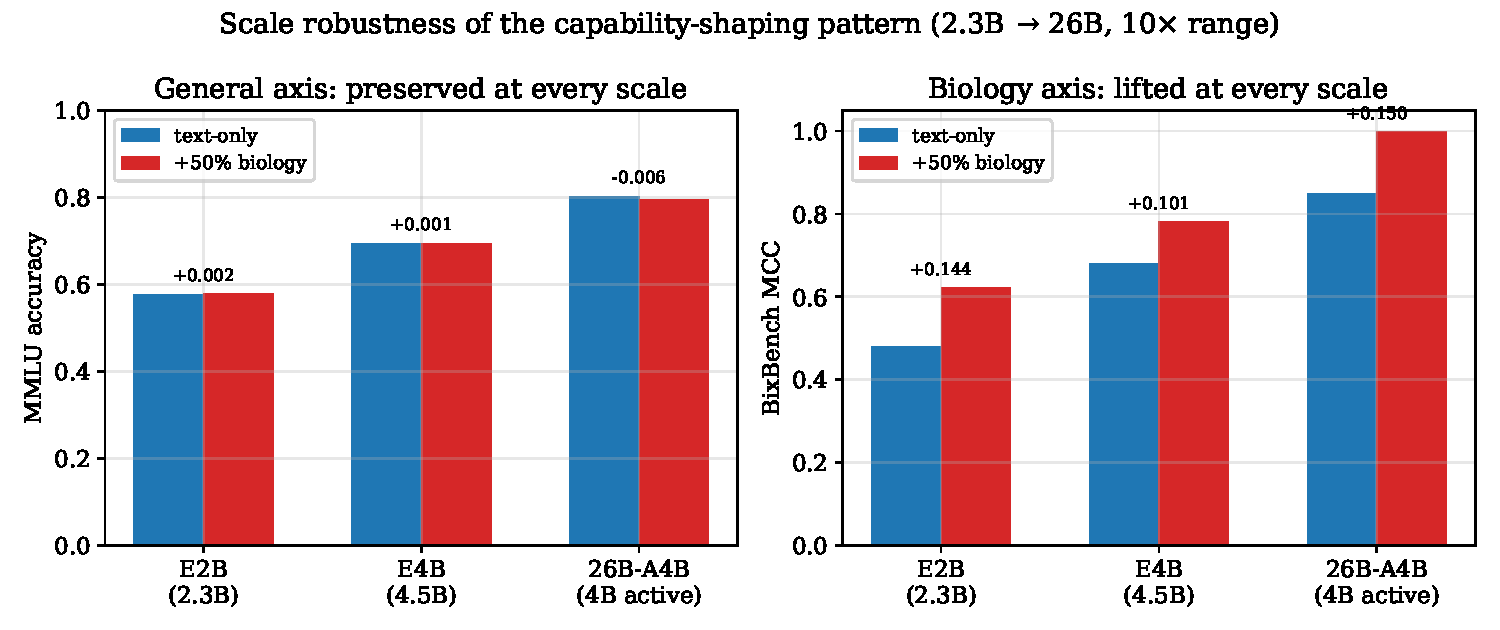
\includegraphics[width=0.92\linewidth]{figs/p4_fig4_scaling.pdf}
\caption{Text-only vs.\ $50\%$-biology contrast at three scales (E2B $2.3$B, E4B $4.5$B, 26B-A4B
$4$B active), same $100$M-token budget and mixture at each size. The general axis (MMLU, left)
is preserved at every scale; the biology axis (BixBench, right) is lifted at every scale.}
\label{fig:p4scaling}
\end{figure}

\subsection{Replay control: uniform mixing was not forgetting anything to begin with}
\label{sec:replay}
A natural objection to \S\ref{sec:phase2} is that the uniformly-shuffled bio50 mixture might be
quietly trading away general capability that a smarter training schedule --- for instance, an
explicit block of pure text placed at the \emph{end} of training, mimicking a replay buffer ---
could recover. We test this directly: holding the total token budget and the overall bio/text
ratio of \texttt{M3-bio50} exactly fixed, we reorder training so the final $10\%$ or $20\%$ of
tokens are a pure-text block (\texttt{R1}, \texttt{R2}), rather than shuffled throughout, and
compare against the fully-shuffled baseline.

Table~\ref{tab:p4replay} and Figure~\ref{fig:p4replay} show the general axis is already flat
across all four conditions ($0.795$--$0.802$ MMLU) --- replay changes nothing on the axis it is
meant to protect, because uniform shuffling was not costing anything there in the first place.
On the biology axis, replay does not help and mildly \emph{hurts}: homology-std falls
monotonically as the replay fraction rises ($0.375\!\to\!0.318\!\to\!0.266$), the sensible
consequence of diverting an increasing fraction of the fixed token budget away from biological
content. BixBench remains near-saturated at $10\%$ replay and dips modestly at $20\%$. We take
this as a clean negative result rather than a null one: at this token budget and model scale,
there is no forgetting problem for an explicit replay schedule to solve, and imposing one has a
small opportunity cost.

\begin{table}[h]\centering\small
\caption{Replay control at fixed $50\%$ biological share, $100$M tokens (26B). Explicit
end-of-training text replay does not change the (already-flat) general axis and mildly reduces
biology-axis performance as the replay fraction rises.}
\label{tab:p4replay}
\begin{tabular}{lccccc}
\toprule
Model & Replay & MMLU & GSM8K & Homology-std & BixBench \\
\midrule
\texttt{M3-bio50} & 0\% (uniform) & 0.796 & 0.861 & \textbf{0.375} & \textbf{1.000} \\
\texttt{R1} & 10\% (tail) & 0.800 & 0.868 & 0.318 & \textbf{1.000} \\
\texttt{R2} & 20\% (tail) & 0.795 & \textbf{0.873} & 0.266 & 0.873 \\
\bottomrule
\end{tabular}
\end{table}

\begin{figure}[h]\centering
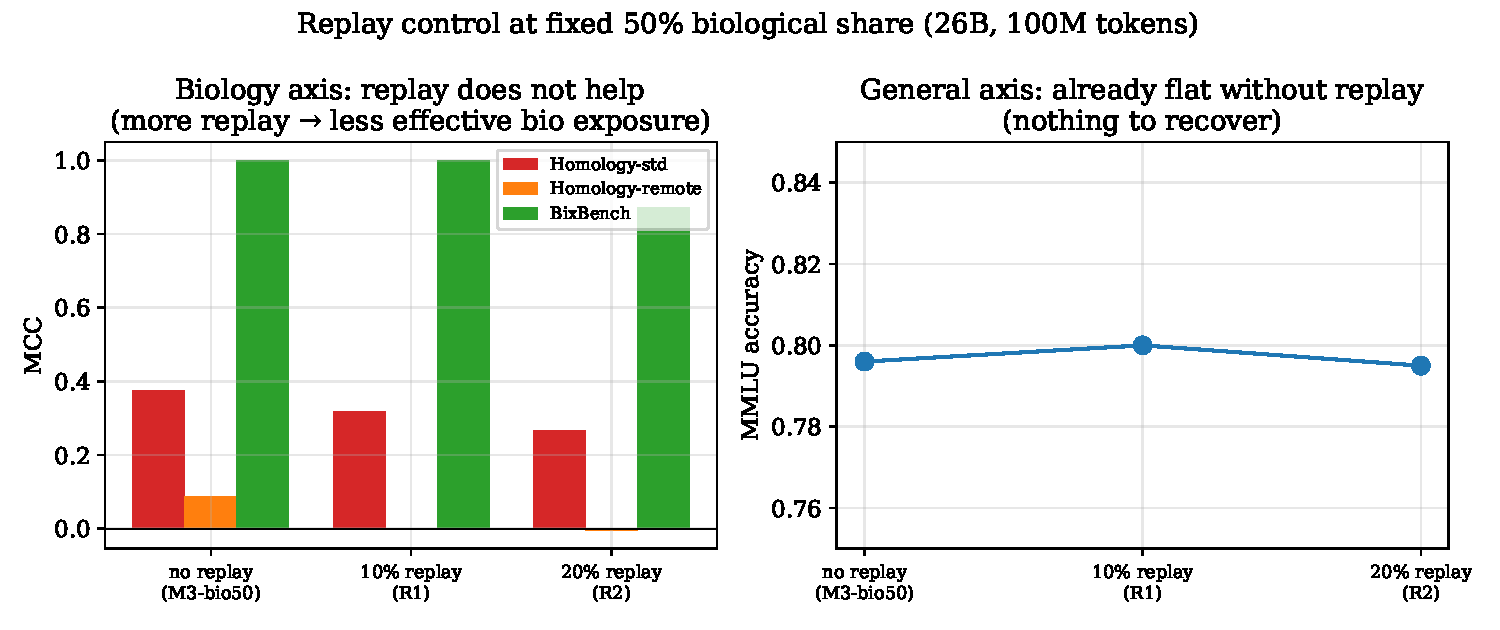
\includegraphics[width=0.92\linewidth]{figs/p4_fig5_replay.pdf}
\caption{Replay control. Left: the biology axis does not benefit from end-of-training text
replay and mildly declines as replay fraction rises. Right: the general axis is already flat
without replay, so there is nothing for replay to recover.}
\label{fig:p4replay}
\end{figure}

\subsection{Router mechanism: capability shaping and routing reorganization are dissociable at LoRA scale}
\label{sec:router}
\S\ref{sec:results} shows that full-parameter CPT ($8.7$B tokens, it-bio~$\to$~BioCPT) shifts
general and biology capability together; does it do so by reorganizing which experts handle
which inputs? We install forward hooks on all $30$ MoE routers and measure the Jensen--Shannon
divergence between expert-routing distributions on protein, DNA, and natural-language prompts,
for every checkpoint in this paper.

The full-CPT lineage reproduces, on our own prompt set, the routing reorganization already
reported for this checkpoint lineage~\citep{wang2026omnigene}: mean biology-vs-language routing
divergence rises from $0.219$ (it-bio, no CPT) to $0.451$ (BioCPT, $8.7$B tokens) --- full CPT
visibly reorganizes which experts serve which modality (Figure~\ref{fig:p4router}). We include
this replication only as a baseline anchor; the new result is what the Phase-2 mixture sweep
shows against it, and it tells a different story. Despite the clear capability dose-response of
\S\ref{sec:phase2} (homology and BixBench rising monotonically with biological share), routing
divergence across \texttt{M0-base} through \texttt{M3-bio50} is flat ($0.376$--$0.385$, no
dose-response) --- and \texttt{M0-base} (\emph{text-only} LoRA CPT) already reaches nearly the
same divergence as the $50\%$-biology model. The composition arm (\texttt{C1}--\texttt{C3})
shows the same flatness. In other words, at $100$M-token LoRA scale, \emph{any} continued
pretraining shifts routing away from the base model by a roughly fixed amount, regardless of
what the training data contains, while the \emph{capability} gained still tracks the biological
share closely. Full-scale CPT ($8.7$B tokens, full-parameter) is what pushes routing divergence
further. We read this as evidence that capability shaping and router-level reorganization are
dissociable mechanisms at the LoRA/$100$M-token regime, converging only at much larger training
budgets --- a genuine nuance rather than a clean confirmation of the naive ``more biology $\to$
more specialized routing'' hypothesis, and one we report as such.

\begin{figure}[h]\centering
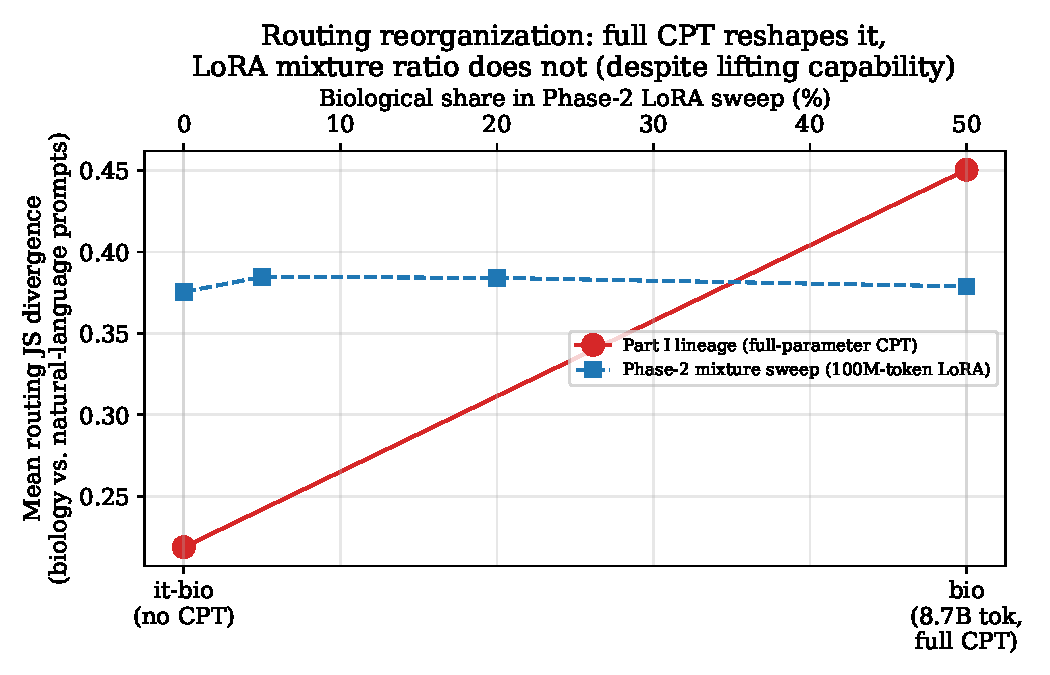
\includegraphics[width=0.78\linewidth]{figs/p4_fig6_router.pdf}
\caption{Routing divergence (biology-vs-language expert allocation) across the full-CPT lineage
(circles, bottom axis) and the Phase-2 LoRA mixture sweep (squares, top axis). Full CPT visibly
reorganizes routing; the LoRA mixture sweep does not show a dose-response in routing despite a
clear one in capability.}
\label{fig:p4router}
\end{figure}
